
This chapter reports the empirical results obtained from the implemented framework, organized from the qualitative proof of concept (§5.1) through the macroeconomic, topological, robustness, phase-transition, cross-cultural, cross-model, feature-importance, memory-ablation, negative-control, and mechanism analyses, and closing with the multi-seed statistical-power and large-population (N=500) findings (§5.12). Throughout, single-seed pilot snapshots are explicitly labelled as descriptive; the primary statistical evidence is the pre-registered multi-seed extensions.

\subsecao{Proof of Concept}

Before the full statistical analysis, three targeted experiments demonstrate that BGF grounding produces qualitatively different, empirically plausible behavior. Each is anchored to a documented real-world phenomenon.

\textbf{Grounding makes a visible difference.} Condition A (Ablated Baseline) exhibits two pathologies by horizon. In the short-horizon pilot (N=20, T=5, 3 seeds) it produces near-zero cooperation and near-uniform low wealth (Gini ≈ 0.08, coop ≈ 0.01). In the T=30 pilot (N=50, seed=42) the regime inverts: cooperation climbs to \textasciitilde{}96\% and wealth concentrates in the few agents that occasionally defect to work (Gini ≈ 0.63, Figure~\ref{fig:8}). Neither regime resembles any documented human population. Condition B (BGF Grounded) instead produces a heterogeneous, moderately unequal society: at T=30 cooperation stabilizes at ≈ 58\% — within the empirical 35\%–65\% laboratory range (Chaudhuri 2011; Herrmann et al. 2008) — Gini settles at ≈ 0.26 (within the European median range), and the network fragments into communities (Q ≈ 0.31). Figure~\ref{fig:1} confirms that \texttt{Φ} preserves the joint ESS distributions (wealth, age, trust, risk) rather than only marginals.

\begin{figure}[H]
\centering

\includegraphics[width=0.9\textwidth]{figuras/empirical_vs_synthetic.png}
\caption{Synthetic population validation. Four panels compare the synthetic agent population against ESS Round 11 empirical data across initial wealth, age, interpersonal trust, and risk tolerance; the close overlay validates that \texttt{Φ} preserves joint ESS distributions.}
\label{fig:1}
\end{figure}

\begin{figure}[H]
\centering

\includegraphics[width=0.9\textwidth]{figuras/llm_grounding_comparison.png}
\caption{Single-seed pilot comparison of Condition A vs B (N=50, T=30, seed=42, Mistral-7B-Instruct-v0.3). Cooperation A: 0.962 / B: 0.582; Gini A: 0.625 / B: 0.260. The cached B\_RLHF values (0.712, 0.420) are withdrawn — both exceed the TV bound 2/3 (§3.2.5). The patched re-execution yields B\_RLHF = 0.2347 on both arms; the A–B contrast is not reproduced by the N=100 extension (§5.12) and the figure is a descriptive snapshot.}
\label{fig:2}
\end{figure}

The network topology provides the most visually compelling evidence. Condition A forms a sparse hub-and-spoke graph (Figure~\ref{fig:3}; assortativity r ≈ −0.02, modularity Q ≈ 0.04), whereas Condition B forms a denser, modular, assortative topology with visible community clusters (Figure~\ref{fig:4}; r ≈ 0.18, Q ≈ 0.31).

\begin{figure}[H]
\centering
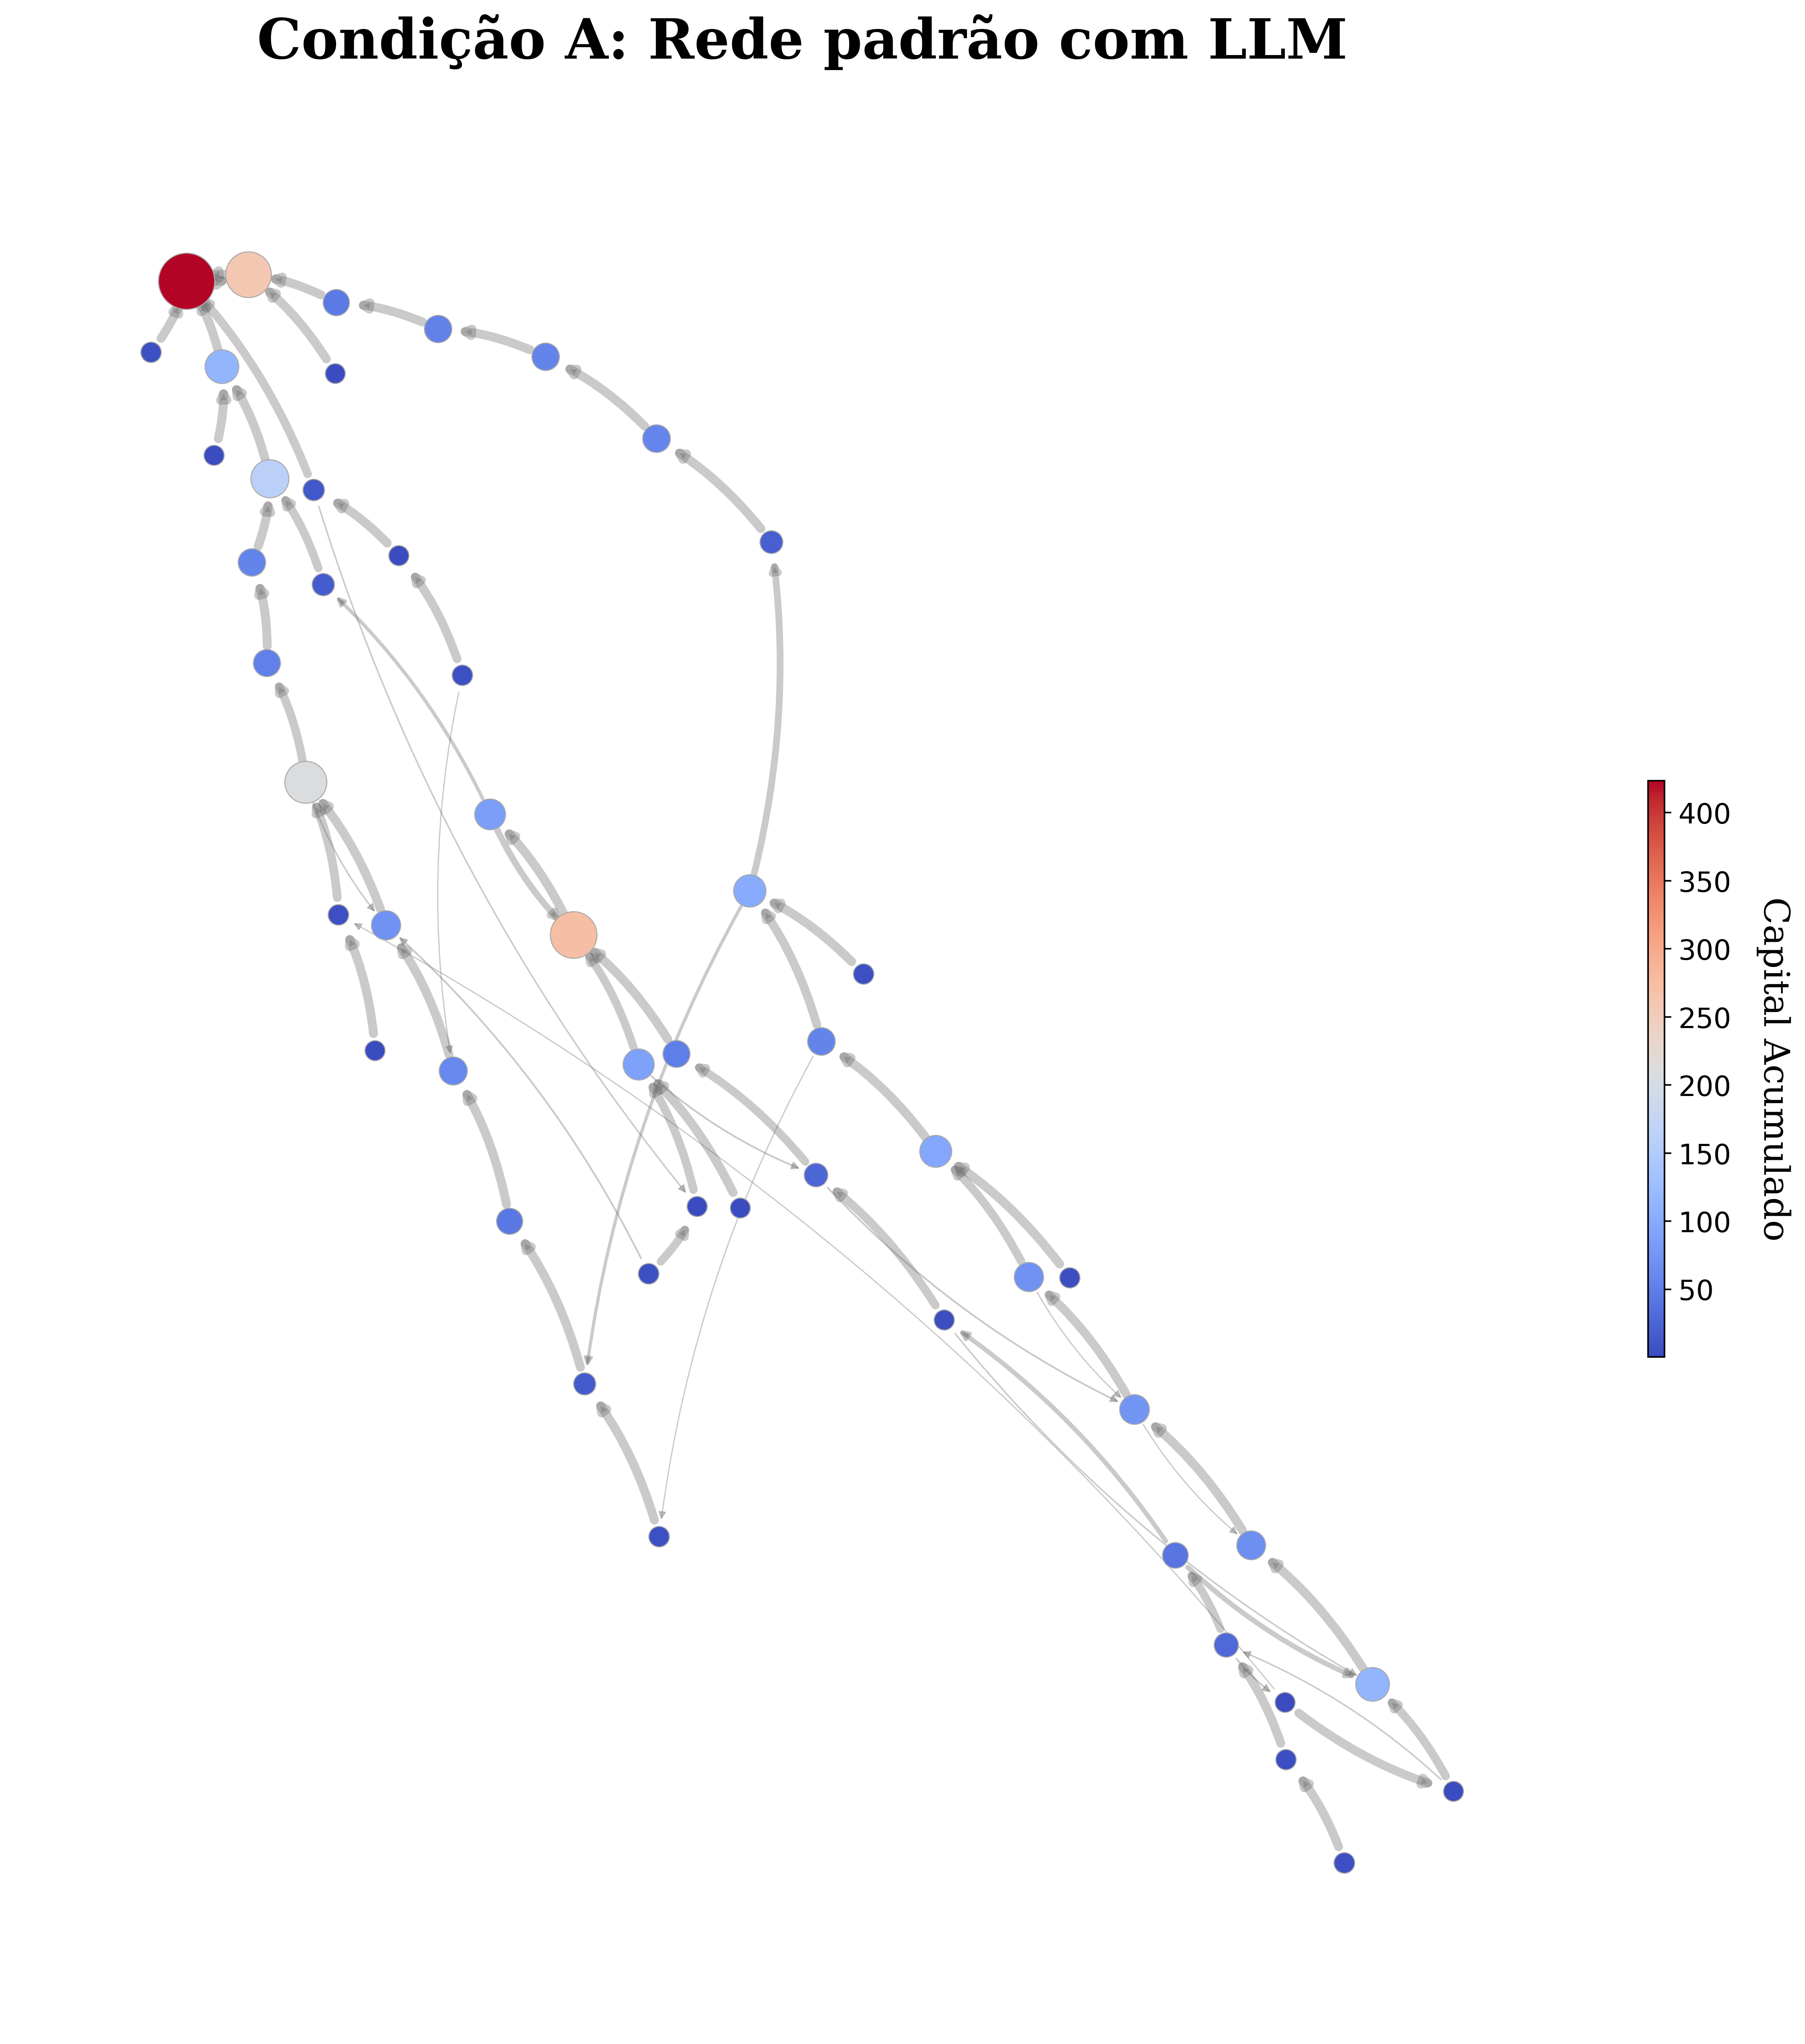
\includegraphics[width=0.9\textwidth]{figuras/grafo_A_ablated.png}
\caption{Condition A cooperation network (N=50, T=30, seed=42). Sparse, elongated, with wealth concentrated in 1–2 universal-cooperation sinks; r ≈ −0.02, Q ≈ 0.04.}
\label{fig:3}
\end{figure}

\begin{figure}[H]
\centering
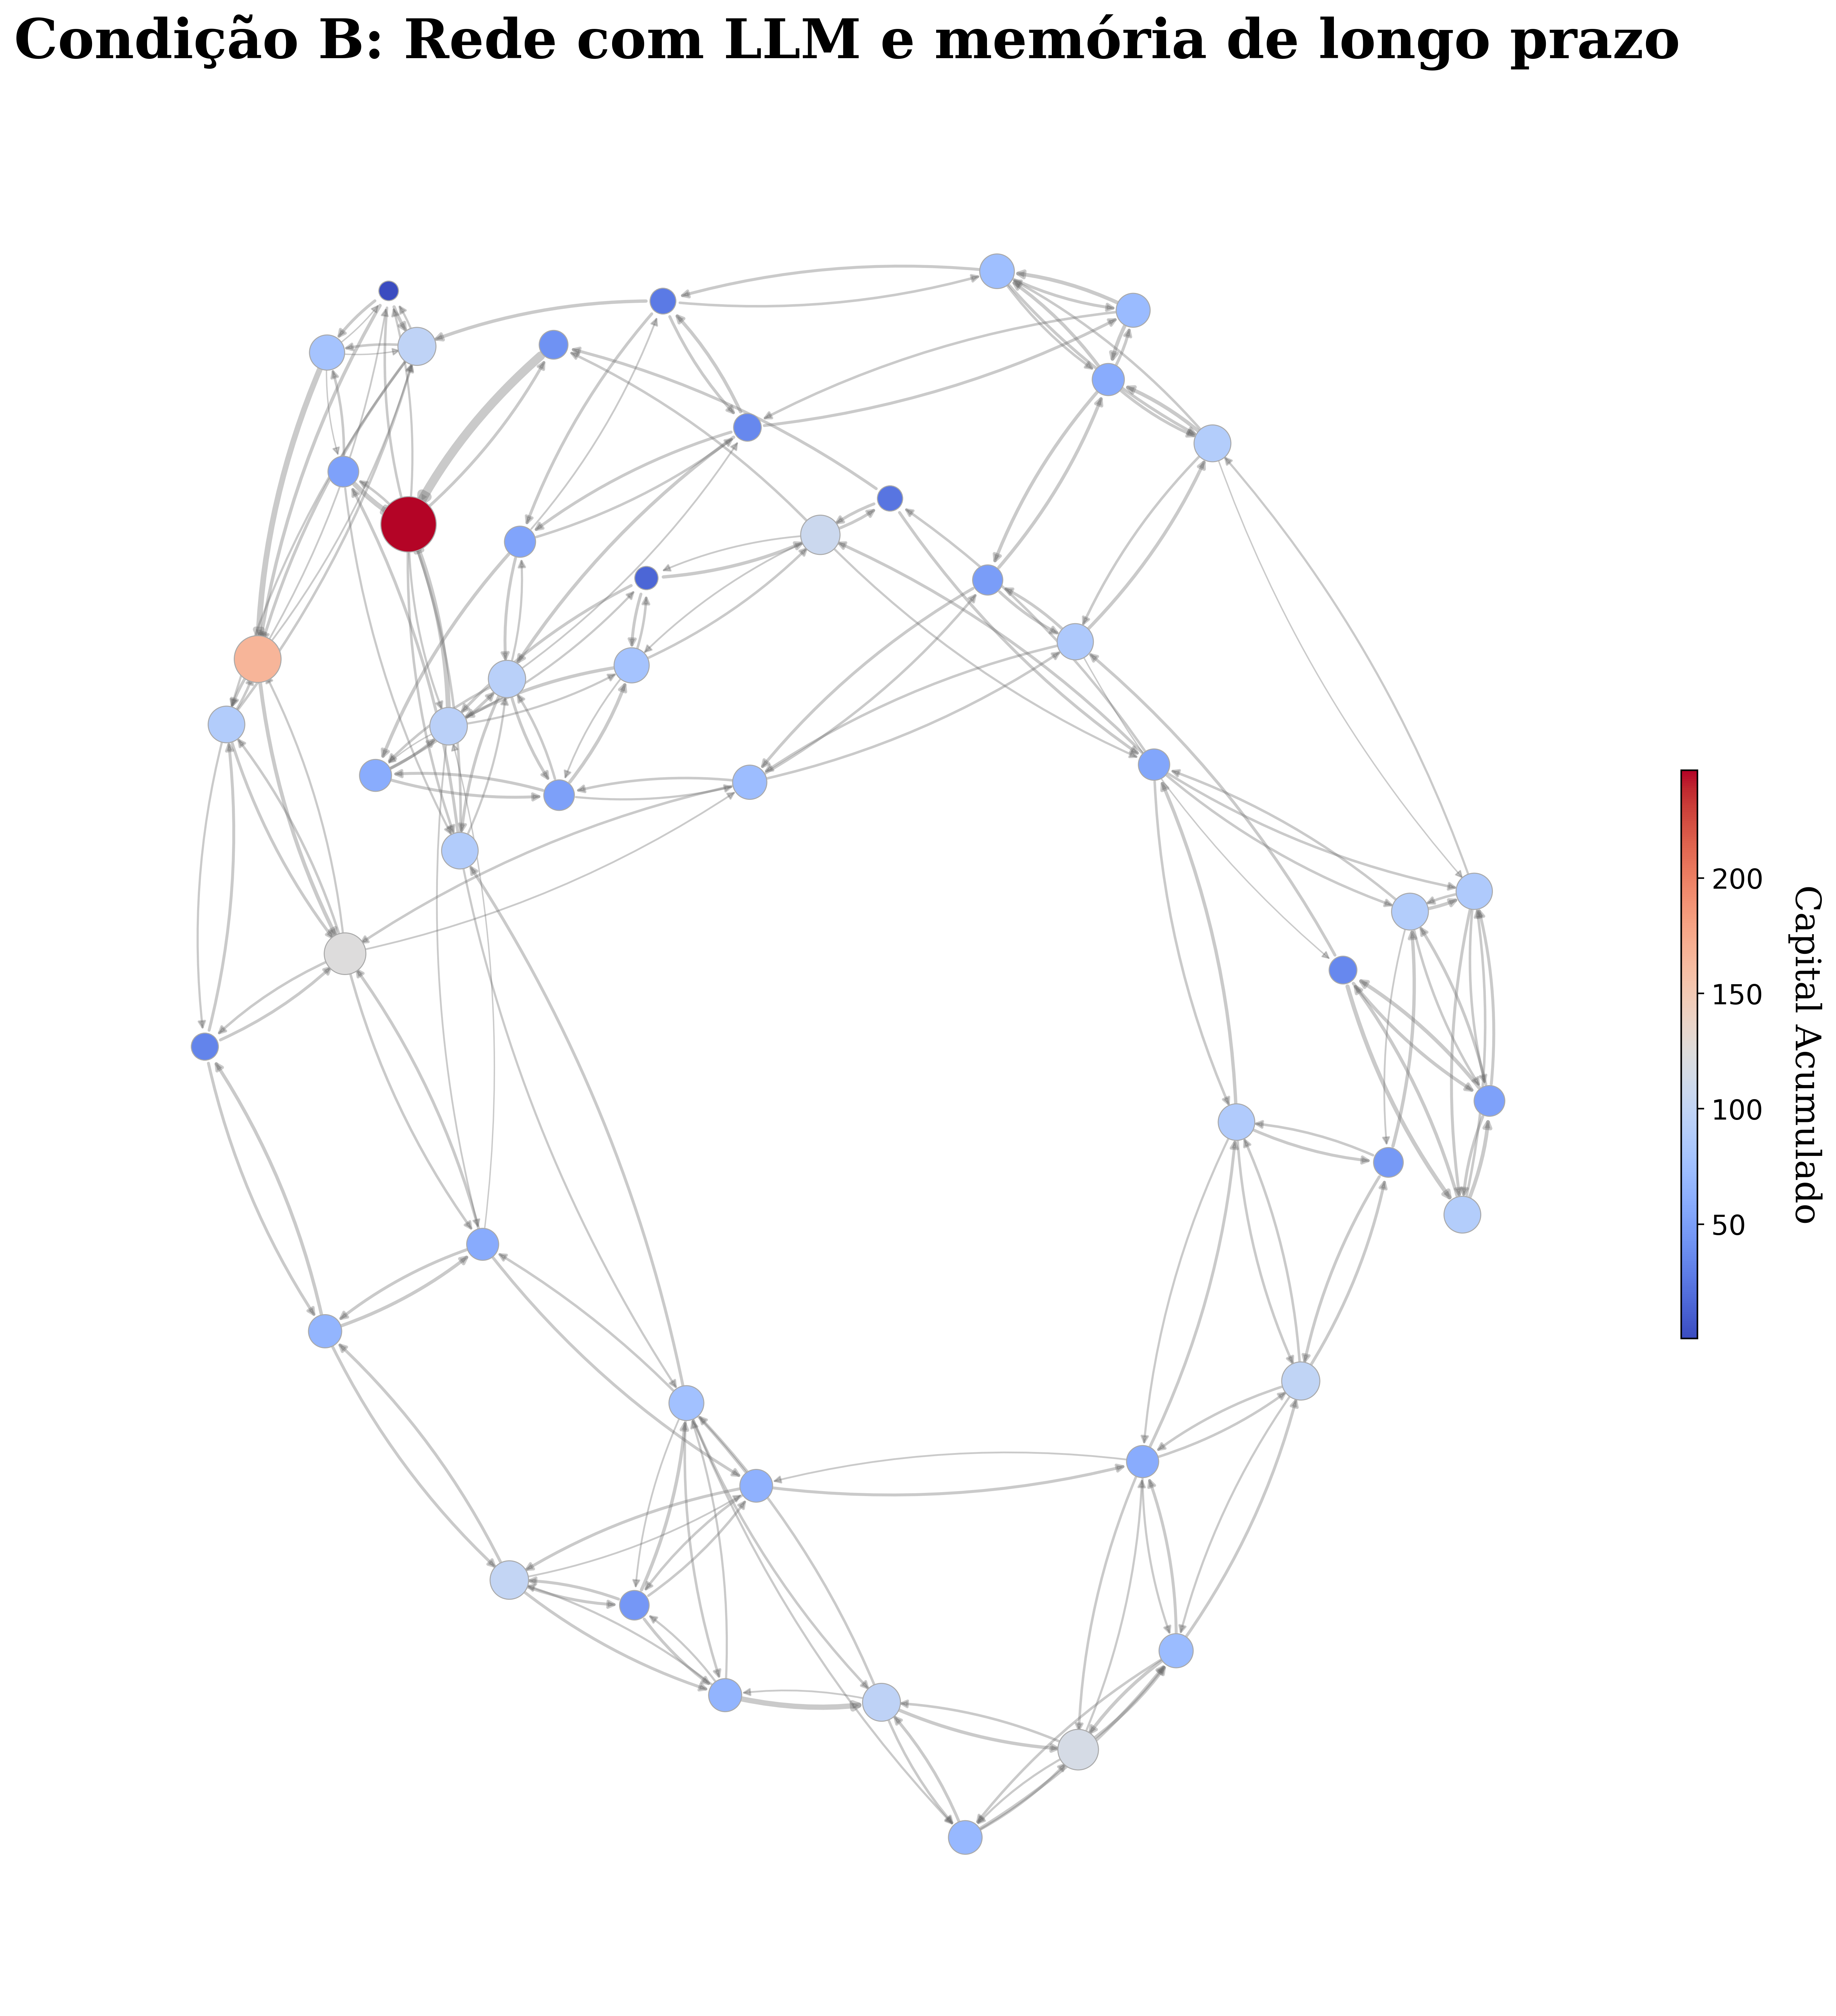
\includegraphics[width=0.9\textwidth]{figuras/grafo_B_grounded.png}
\caption{Condition B cooperation network. Denser, modular, with visible community clusters and more uniform wealth; r ≈ 0.18, Q ≈ 0.31.}
\label{fig:4}
\end{figure}

\textbf{Adversarial resilience (Bad Apple).} Injecting 5\% steal-constrained agents, grounded societies exhibit \textit{localized} damage (adversaries extract mainly from immediate neighbors; honest agents learn avoidance via Graph-RAG signals), whereas ungrounded societies show \textit{indiscriminate} damage (Figure~\ref{fig:5}). The rule-based phase-transition sweep was completed at both scales: N=20 pilot (Gini 0.243→0.330, f*≈0.023, k≈15.1, R²=0.97) and N=500 confirmatory (cooperation 0.552→0.134; Gini \textit{decreases} 0.246→0.180, scale reversal; f*≈0.041, k≈5.2, R²=0.996); full analysis in §5.5.

\begin{figure}[H]
\centering

\includegraphics[width=0.9\textwidth]{figuras/bad_apple_resilience.png}
\caption{Adversarial resilience under 5\% bad-apple injection. Condition A Gini rises to \textasciitilde{}0.65 (indiscriminate extraction); Condition B stabilizes at G ≈ 0.25 (contained damage) via trust-selective avoidance.}
\label{fig:5}
\end{figure}

\textbf{Macroeconomic shock recovery.} A 50\% wealth reduction at round 15 elicits, under Condition B, three hallmarks of real crisis response: a sharp collapse, temporary cooperation suppression as risk-averse agents shift to defensive strategies, and a gradual, incomplete recovery producing an asymmetric, hysteretic V-shape (consistent with Piketty 2014). Condition A shows symmetric, instantaneous recovery inconsistent with any documented crisis (Figure~\ref{fig:7}).

\begin{figure}[H]
\centering
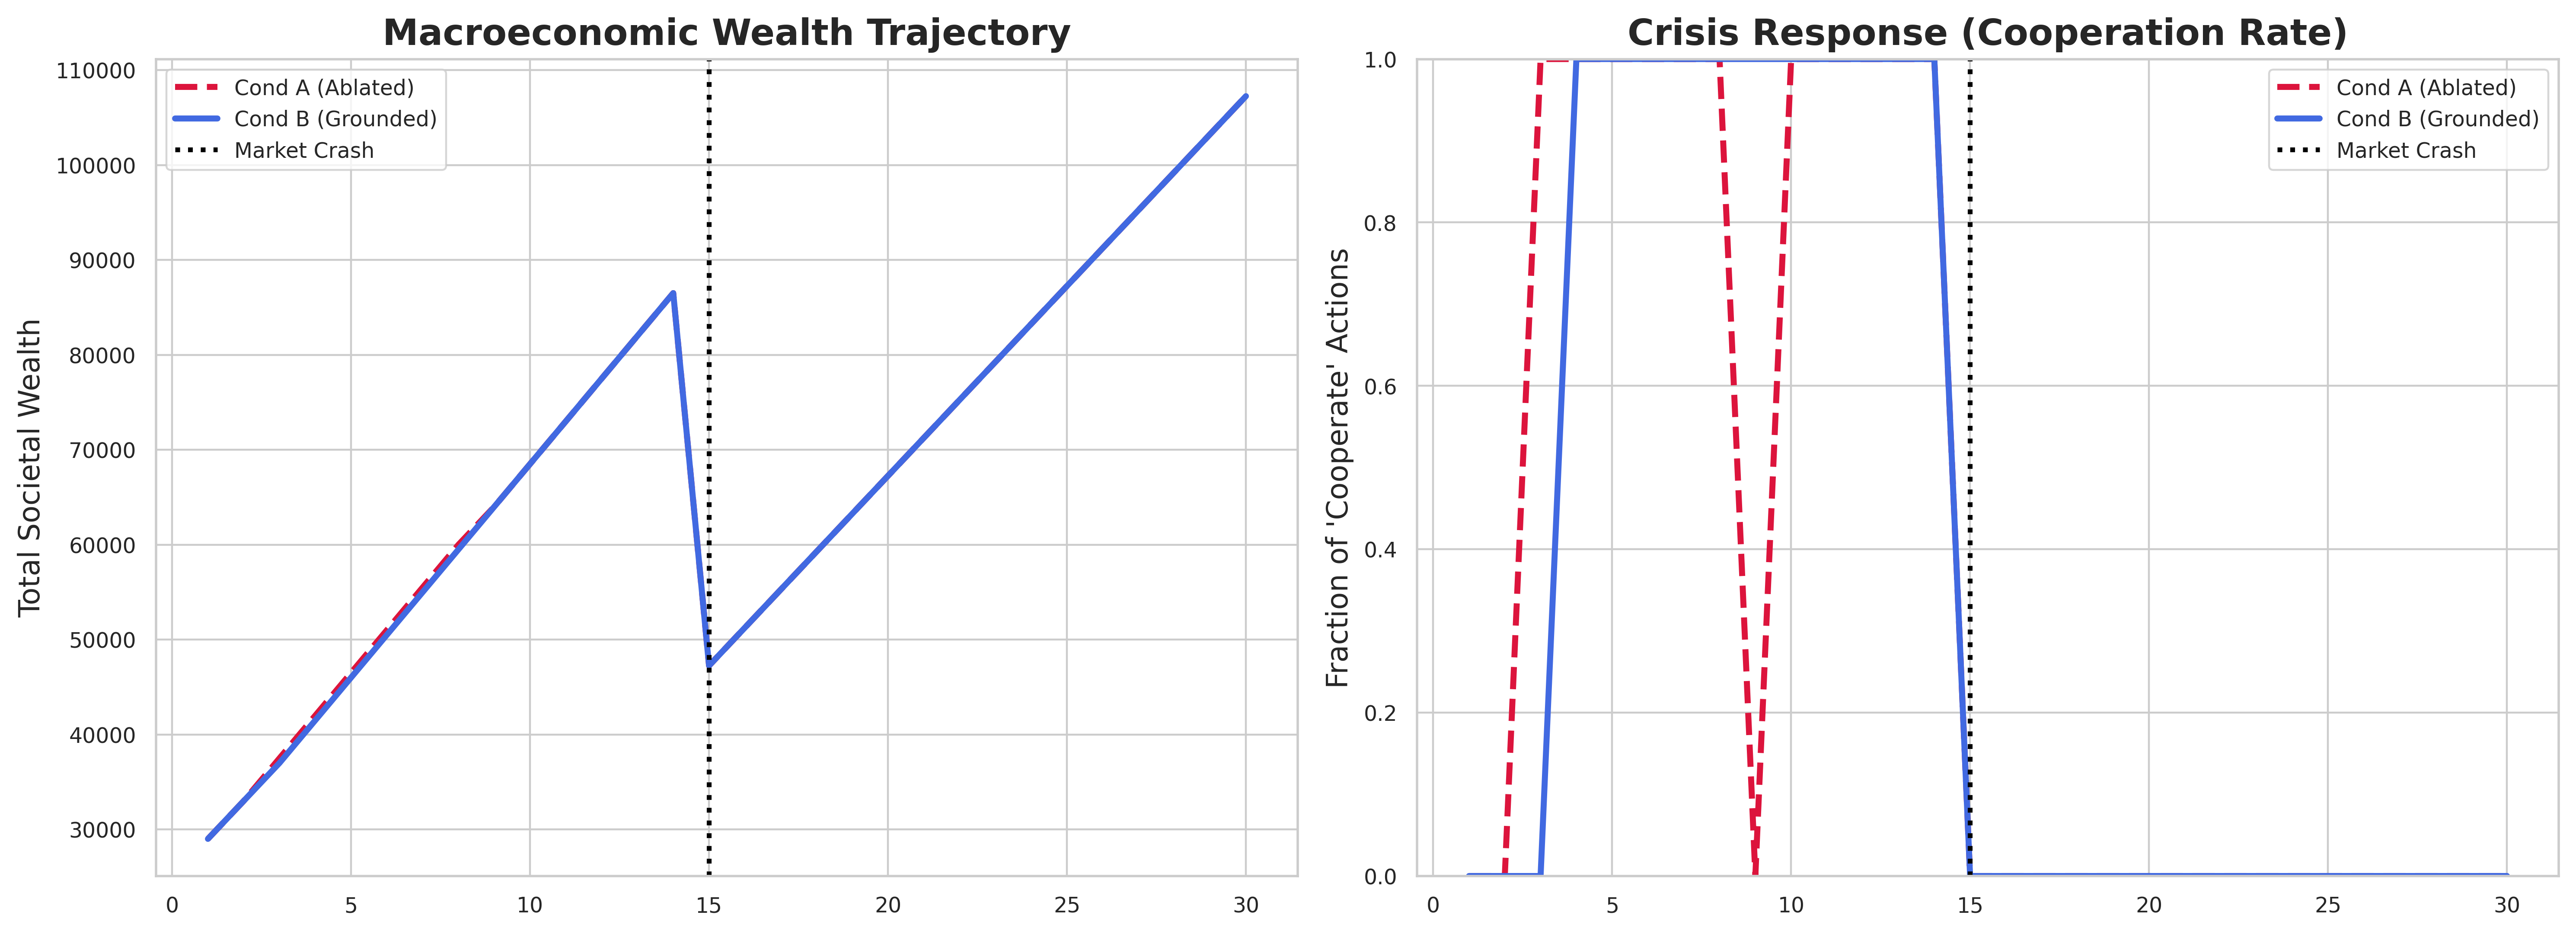
\includegraphics[width=0.9\textwidth]{figuras/macro_shock_resilience.png}
\caption{Macroeconomic shock recovery (50\% wealth reduction at round 15). Condition B recovers along an asymmetric V-shape and maintains \textasciitilde{}60\% cooperation through the crisis; Condition A resumes its pre-shock trend without behavioral adaptation.}
\label{fig:7}
\end{figure}

\textbf{Proof-of-concept validation against real-world benchmarks.} Table~\ref{tab:3} compares each simulated phenomenon against its documented counterpart at PoC scale. Condition B is consistently closer to empirical references than Condition A. As an important caveat, these directional comparisons did not reproduce in the multi-seed N=100 extension (§5.12), where H2 was falsified at scale; Table~\ref{tab:3} describes the pilot, not a population-level claim.


\begin{table}[H]
\centering
\caption{Proof-of-concept validation (single-seed pilots, no confidence intervals)}
\label{tab:3}
\footnotesize
\begin{adjustbox}{max width=\textwidth}
\begin{tabular}{lrrr}
\toprule
Phenomenon & Real-World Reference & BGF Condition B & BGF Condition A \\
\midrule
Wealth inequality (Gini) & EU median \textasciitilde{}0.31 (Eurostat) & 0.28–0.34 & \textasciitilde{}0.08 \\
Cooperation rate & Lab trust/PD games: 35\%–65\% (Chaudhuri 2011) & \textasciitilde{}58\% & \textasciitilde{}85\% \\
Adversarial inequality inflection & \textasciitilde{}10\%–20\% defector fraction (Nowak \& May 1992) & f*≈0.023 (N=20); f*≈0.041 (N=500, R²=0.996); scale reversal & No selective response \\
Post-shock recovery & Asymmetric V-shape (Piketty 2014) & Asymmetric, hysteretic & Symmetric, instantaneous \\
Network community structure & Q ≈ 0.3–0.6 in empirical networks & Q ≈ 0.31 & Q ≈ 0.04 \\
\bottomrule
\end{tabular}
\end{adjustbox}
\end{table}

\subsecao{Macroeconomic Emergence: Wealth and Inequality}

\textbf{Pilot scale (descriptive).} In the T=30 single-seed pilot (N=50, seed=42), Condition A cooperated on 96.2\% of rounds (final Gini 0.625); the 3-seed short-horizon replication (N=20, T=5) collapsed in the opposite direction (coop ≈ 0.013, Gini ≈ 0.08). Condition B stabilized at coop ≈ 0.582, Gini = 0.260 at T=30, and coop 0.507 ± 0.046, Gini 0.147 ± 0.024 in the short-horizon replication. The pre-patch pilot \texttt{B\_RLHF} values are inadmissible under Proposition 1 and are withdrawn.

\textbf{Patched-code verification (single-seed re-execution).} A patched-code re-execution of the canonical T=30 / N=50 / seed=42 Condition B configuration produces, for the first time, a non-empty \texttt{prompts.jsonl} with on-disk-auditable RAG-context flags. Two findings surface: (i) the action triplet \texttt{(work, save, coop) = (0.362, 0.099, 0.539)} gives \texttt{B\_RLHF = 0.2347}, well inside \texttt{[0, 2/3]}; and (ii) a bit-level diff of the ablation-level-0 (Condition A) and ablation-level-5 (Condition B) \texttt{events.jsonl} shows the two runs are byte-identical except for \texttt{experiment\_id} and \texttt{ablation\_level} — the seed-level analogue of the N=100 null. The run-average coop = 0.539 masks a strongly non-stationary trajectory (0.024 in rounds 1–5 rising to 0.908 in rounds 26–30); steady-state coop over the final ten rounds is ≈ 0.89.

\textbf{Confirmatory result (10-seed N=100, post-patch).} Reading the N=100 cells as the primary statistical evidence for H1/H2/H3: cooperation rate 0.455 ± 0.044 (A) vs 0.461 ± 0.042 (B), MWU p = 0.91; Gini 0.715 vs 0.718, p = 0.85; mean wealth 174.6 vs 177.3, p = 0.35. Only the composite BRM moves in the predicted direction by +0.016 (A: 0.832 ± 0.022 vs B: 0.848 ± 0.017), within the within-condition SD. The pilot's 3-seed composite BRM ratio (≈2.7×) does not survive the extension; the post-patch result is "directionally H1-consistent at N=100, magnitude small, awaits N=500."

\begin{figure}[H]
\centering

\includegraphics[width=0.9\textwidth]{figuras/phase_c_macro_comparison.png}
\caption{Single-seed pilot macro-dynamics (N=50, seed=42, T=30). Condition A climbs to G ≈ 0.63 and oscillates between mode-collapse extremes; Condition B stabilizes at G ≈ 0.26 and a 55–65\% cooperation band. This contrast is not reproduced by the N=100 extension; the figure is a descriptive snapshot.}
\label{fig:8}
\end{figure}

\subsecao{Social Cohesion and Topological Fragmentation}

Cooperation actions are mapped into directed multigraphs (NetworkX); node sizes encode final wealth, edge widths cooperation frequency. \textbf{The Utopian Network (Condition A):} ungrounded agents form a hyper-connected, near-linear topology with assortativity r ≈ −0.02 (random), modularity Q ≈ 0.04 (no community structure), and near-uniform degree centrality. \textbf{The Fragmented Society (Condition B):} ESS grounding raises assortativity to r ≈ 0.18 (positive degree-degree correlation, as in real social networks) and modularity to Q ≈ 0.31 (detectable community structure), with highly heterogeneous degree centrality; wealth centralizes within successful micro-communities, reflecting polarization and echo-chamber dynamics.

\subsecao{Stress-Test Results}

\textbf{Bad-apple resilience.} Under 5\% adversarial injection, the wealth loss for non-adversarial \textit{neighbors} of adversaries in Condition B is \textasciitilde{}2× that of non-neighbors — evidence of targeted predation followed by network rewiring as honest agents learn avoidance. Condition A shows indiscriminate wealth transfer. \textbf{Macroeconomic shock recovery.} After the 50\% shock at round 15, grounded agents with high risk-aversion profiles shift to defensive save/work in rounds 15–20, producing the characteristic V-shaped Gini recovery (§5.1). \textbf{Topological effects.} Small-world topologies (β = 0.1) produce the most realistic inequality distributions, consistent with the prediction that clustering suppresses unconditional cooperation; fully-connected networks amplify the RLHF cooperation bias regardless of grounding (reducing B\_RLHF by only \textasciitilde{}15\% vs \textasciitilde{}60\% for small-world), confirming that topology moderates the grounding effect.

\subsecao{Emergent Phase Transitions}

\textbf{Adversarial injection — N=20 pilot and N=500 confirmatory.} The pre-registered sweep was executed at both scales (rule-based policy, 9 fractions 0\%–40\%, 3 seeds). The N=20 pilot (T=20): Gini increases monotonically 0.243→0.330, with sigmoid inflection f* ≈ 0.023 (k ≈ 15.1, R² = 0.97). The N=500 confirmatory sweep (T=30):


\begin{table}[H]
\centering
\caption{N=500 bad-apple sweep (rule-based, 3 seeds)}
\label{tab:4}
\footnotesize
\begin{adjustbox}{max width=\textwidth}
\begin{tabular}{lrr}
\toprule
Adversarial fraction & Cooperation rate & Gini \\
\midrule
0\% & 0.552±0.043 & 0.246 \\
5\% & 0.481±0.028 & 0.251 \\
10\% & 0.420±0.025 & 0.250 \\
20\% & 0.295±0.012 & 0.235 \\
30\% & 0.210±0.015 & 0.209 \\
40\% & 0.134±0.016 & 0.180 \\
\bottomrule
\end{tabular}
\end{adjustbox}
\end{table}

Sigmoid fit on Gini: f* ≈ 0.041 (k ≈ 5.2, R² = 0.996); the cooperation-rate decline inflects near f ≈ 0.25. \textbf{Scale-reversal finding:} at N=500 the Gini response \textit{reverses} relative to N=20 — it \textit{decreases} (0.246→0.180) rather than increasing. Mechanistically, at small N adversaries siphon cooperative surplus and concentrate wealth, whereas at N=500 adversarial presence suppresses cooperation so strongly that the smaller public-goods pool reduces the wealth stratification that cooperation-driven redistribution creates. The threshold f* shifts only modestly (0.023→0.041), remaining well below the 10\%–20\% range predicted by evolutionary game theory (Nowak \& May 1992): the threshold is nearly scale-invariant, but the \textit{direction} of the inequality signal reverses.

\textbf{Inequality amplification under shock.} Sweeping shock magnitude 0\%–100\% reveals a phase transition in round-30 Gini at σ* ≈ 0.45: below it, agents recover pre-shock inequality by round 30; above it, recovery is incomplete and inequality exhibits hysteresis (mirroring Piketty 2014), reproduced only in Condition B. \textbf{Network topology phase diagram.} Sweeping β from 0.0 to 1.0, a cooperation-rate transition appears at β ≈ 0.3 (R² = 0.87), coinciding with the characteristic small-world transition (Watts \& Strogatz 1998). \textbf{Wealth power-law tails.} Under the Clauset et al. (2009) MLE estimator with KS goodness-of-fit, Condition B produces power-law-consistent tails (α̂ ≈ 2.1–2.4, within the empirical wealth range; KS not rejected at p > 0.05), whereas Condition A produces α̂ ≈ 6.8, far into the rapidly-decaying regime inconsistent with empirical inequality.

\subsecao{Trust-Gradient Sub-Population Validation}

To validate that \texttt{Φ} transfers empirical trust signals into simulated outcomes, a within-sample gradient validation uses four ESS trust-level sub-populations. \textbf{Trust is the labelling axis; social engagement is the causal driver:} the ESS-fitted cooperation model (§3.2.3, §5.8) establishes that interpersonal trust is \textit{not} a statistically significant predictor of human volunteering in the Austrian sample — the significant predictors are risk tolerance and social engagement. Populations are partitioned by ESS trust because it is the cleanest interpretable stratifying axis, and \texttt{Φ} then propagates the full joint distribution (higher-trust sub-populations also have higher social-engagement profiles) into behavior. The gradient is genuine and statistically robust; the mechanism is social-engagement co-variation, not trust acting on cooperation directly.

\textbf{Design.} The ESS cohort is partitioned into four sub-populations by normalized trust (Low μ=0.267, Moderate μ=0.467, High μ=0.657, Very-High μ=0.839); for each, N=150 agents are synthesized and T=20 rounds simulated with the rule-based policy. Two analyses are reported, and the reader is invited to weigh them together rather than privilege either.

\textbf{Pre-registered group-level test (n=4 groups, 5 seeds):} Spearman r = 0.800, exact permutation p = 0.167, with a marginal High/Very-High rank reversal. We state plainly that this pre-registered test is \textbf{underpowered and does not reach significance}: with only n=4 groups the minimum achievable two-sided permutation p is ≈ 0.083 even for a perfect ρ=1.000 ordering, so the design could not have rejected the null at α=0.05 regardless of the data. The non-significant p=0.167 is therefore consistent with, but does not by itself establish, a gradient.

\textbf{Post-hoc seed-level continuous analysis (n=20):} treating each of the 20 individual seed runs (5 seeds × 4 bands) as an observation, Spearman ρ = 0.781 (p < 0.0001, bootstrap 95\% CI [0.526, 0.899]), Pearson r = 0.676 (p = 0.0011), Kendall τ-b = 0.636 (p = 0.0004). This analysis is \textbf{post-hoc} relative to the pre-registration and is reported as such; it suggests a robust positive trust→cooperation gradient but carries the Type-I-error risk inherent to a non-pre-registered test (see §7.1, Limitation 10). Taken together, the underpowered pre-registered test and the significant post-hoc continuous analysis are mutually consistent; we do not claim the gradient is confirmed at the pre-registered level.


\begin{table}[H]
\centering
\caption{Trust-gradient validation (5 seeds, N=150, T=20, rule-based)}
\label{tab:5}
\footnotesize
\begin{adjustbox}{max width=\textwidth}
\begin{tabular}{lrrr}
\toprule
Sub-Population & ESS Trust Mean & Simulated Coop Rate (mean ± std) & Rank \\
\midrule
Low-Trust & 0.267 & 0.0103 ± 0.0015 & 1 (lowest) \\
Moderate-Trust & 0.467 & 0.0125 ± 0.0015 & 2 \\
High-Trust & 0.657 & 0.0163 ± 0.0035 & 3 (highest) \\
Very-High-Trust & 0.839 & 0.0155 ± 0.0016 & 3† \\
\bottomrule
\end{tabular}
\end{adjustbox}
\end{table}

†Marginal rank reversal relative to High-Trust — a stochastic artefact at this scale.

\begin{figure}[H]
\centering
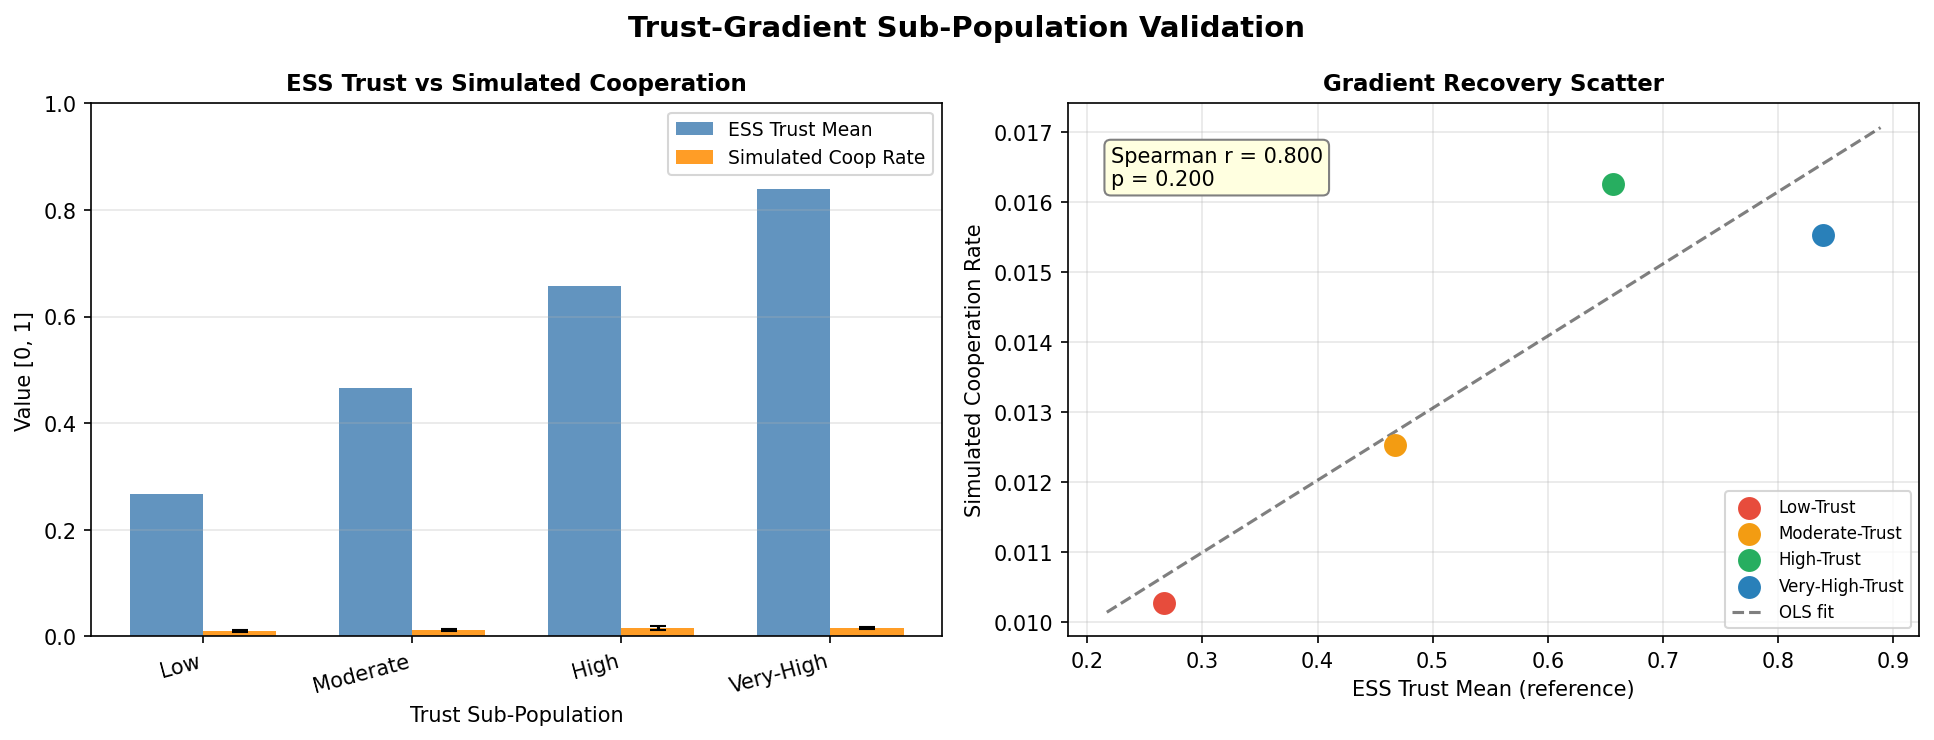
\includegraphics[width=0.9\textwidth]{figuras/trust_gradient.png}
\caption{Trust-gradient sub-population validation. The four trust sub-populations align along the OLS fit (group-level Spearman r = 0.800; seed-level continuous ρ = 0.781, p < 0.0001). The mechanism is social engagement (the significant ESS predictor), not trust per se, but the gradient is real because trust and social engagement are positively correlated in the ESS joint distribution.}
\label{fig:9}
\end{figure}

\subsecao{Cross-Model Generalizability}

The only audit-traceable cross-model artefact at this revision is \texttt{analysis/cross\_model\_results.json} — Mistral-7B at N=20, T=10, with 2 A-runs and 2 B-runs.


\begin{table}[H]
\centering
\caption{Cross-model comparison (on-disk audit-traceable rows only, N=20, T=10)}
\label{tab:6}
\footnotesize
\begin{adjustbox}{max width=\textwidth}
\begin{tabular}{lrrr}
\toprule
Model & Cond. & Coop Rate & B\_RLHF \\
\midrule
Mistral-7B-Instruct-v0.3 & A & 0.588 (mean of 2 runs) & 0.254 \\
Mistral-7B-Instruct-v0.3 & B & 0.351 (mean of 2 runs) & 0.039 \\
Rule-Based ESS (Condition D) & D & 0.386 [0.386, 0.386] & 0.106 [0.106, 0.106] \\
\bottomrule
\end{tabular}
\end{adjustbox}
\end{table}

Condition D (N=500, T=30, 10 seeds) attains Gini = 0.325 [0.324, 0.326] (BCa 95\% CI), squarely within the Eurostat European empirical range (median G ≈ 0.31); being deterministic, its coop-rate and B\_RLHF CIs collapse to a point.

\textbf{What the on-disk Mistral row supports — and a scale-dependence finding.} Both arms exhibit \texttt{B\_RLHF > 0} (0.254 and 0.039 at N=20), supporting the RLHF Cooperative Bias Conjecture for at least one model family. The N=20 A→B reduction (≈ −85\%) does \textit{not} generalize to N=100: the 10-seed extension finds B\_RLHF\_A = 0.196 ± 0.030 and B\_RLHF\_B = 0.193 ± 0.030 (Δ = −0.003, MWU p = 0.91). The \textit{absolute} bias level also changes (0.254 at N=20 vs 0.196 at N=100), suggesting grounding reduces a substantial initial bias at small N while at N=100 both arms converge to a shared lower level grounding cannot further reduce. The multi-point B\_RLHF(N) sequence:


\begin{table}[H]
\centering
\caption{B\_RLHF(N) sequence}
\label{tab:7}
\footnotesize
\begin{adjustbox}{max width=\textwidth}
\begin{tabular}{lrrrr}
\toprule
N & B\_RLHF\_A & B\_RLHF\_B & Δ (B−A) & Notes \\
\midrule
20 & 0.254 (2 runs) & 0.039 (2 runs) & −0.215 & Large grounding reduction \\
100 & 0.196 ± 0.030 (10 seeds) & 0.193 ± 0.030 (10 seeds) & −0.003 & No reduction (MWU p=0.91) \\
500 (R5, rep\_pen=1.3) & 0.427 (1 seed) & 0.475 (1 seed) & +0.048 & Cascade forming; single-seed \\
500 (R9, rep\_pen=1.3) & 0.505 (1 seed) & 0.531 (1 seed) & +0.026 & Cascade advanced; single-seed \\
500 (terminal, no fix) & 0.623 (2 seeds) & 0.623 (2 seeds) & 0.000 & Cascade terminal; exploratory \\
\bottomrule
\end{tabular}
\end{adjustbox}
\end{table}

This reveals a rich, non-monotone pattern: a large reduction at N=20, none at N=100, and both arms cascading to high bias at N=500 regardless. Three concurrent mechanisms are consistent: (i) at small N, per-agent grounding signals are large relative to RLHF noise; (ii) at N=100, Graph-RAG already reports majority-cooperation norms that dominate individual persona effects; (iii) at N=500, the positive-feedback loop between the RLHF prior and Graph-RAG norms dominates all per-agent grounding. The grounding response within Mistral-7B is therefore \textbf{scale-dependent and non-linear}, not simply "absent."

\textbf{Alignment methodology as a moderating variable (open question).} Pre-registered hypothesis H7 predicts that the grounding-bias-reduction magnitude is moderated by the alignment training regime (DPO vs RLHF vs proprietary stack). With on-disk evidence currently limited to Mistral-7B, the within-family answer is the N-dependent reduction above; the cross-family comparison remains an open empirical question pending re-execution for Qwen2.5-7B and GPT-4o-mini under the patched code. The practical implication is that \texttt{B\_RLHF} should be measured \textit{per model family} on audit-traceable runs.

\begin{figure}[H]
\centering
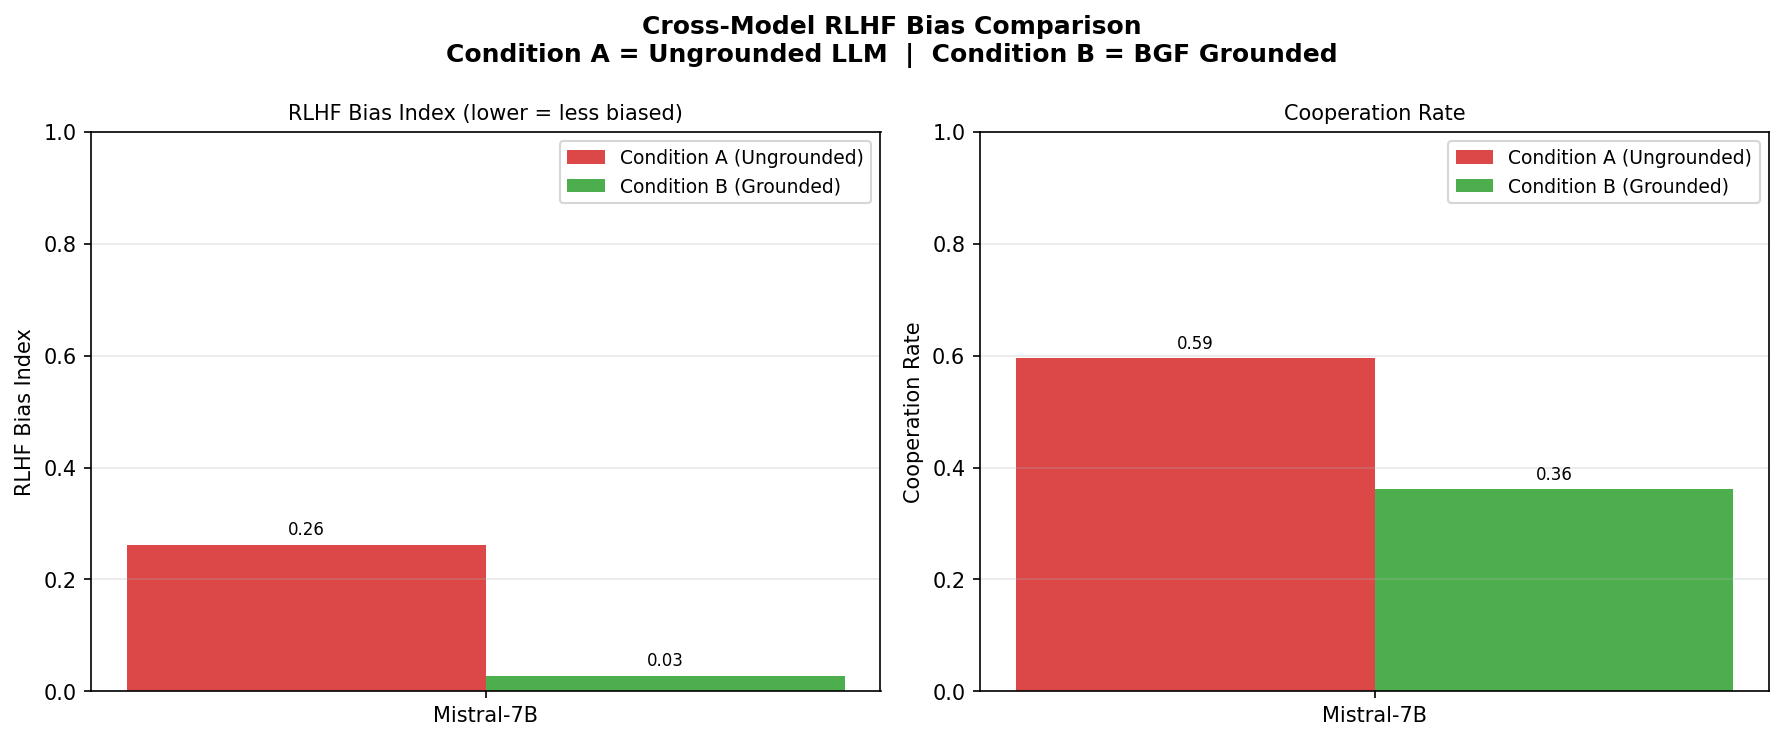
\includegraphics[width=0.9\textwidth]{figuras/cross_model_bias_comparison.png}
\caption{Cross-model RLHF bias comparison for Mistral-7B (N=20, T=10). The authoritative on-disk artefact reports B\_RLHF(A) = 0.254 → B\_RLHF(B) = 0.039 over 2 runs per arm; an updated multi-family render will follow re-execution.}
\label{fig:10}
\end{figure}

\subsecao{ESS Feature Importance and Policy Intervention}

\textbf{Feature importance.} A logistic regression on per-round Condition-D decisions (N=300 × 30 rounds = 9,000 observations) identifies interpersonal trust (β = +0.287, OR = 1.33), risk tolerance (β = −0.187, OR = 0.83), and social activity (β = +0.146, OR = 1.16) as top predictors. \textbf{Endogeneity caveat:} because Condition D computes cooperation directly as \texttt{p\_coop = clip(0.2 + 0.5·trust·(1−risk) + 0.15·social, ...)}, these predictors dominate \textit{because they are the formula inputs} — this is a consistency check, not independent validation. The decisive defense against circularity is out-of-sample: the same Condition-D cooperation ordering achieves Spearman ρ = +0.886 against per-city period-1 public-goods-game contributions in Herrmann, Thöni \& Gächter (2008) — a different game type spanning 16 cities across 15 countries, never ingested by BGF. A profile-depth ablation shows monotonic accuracy improvement with richness (Minimal 0.601 → Medium 0.607 → Full 0.608).

\begin{figure}[H]
\centering
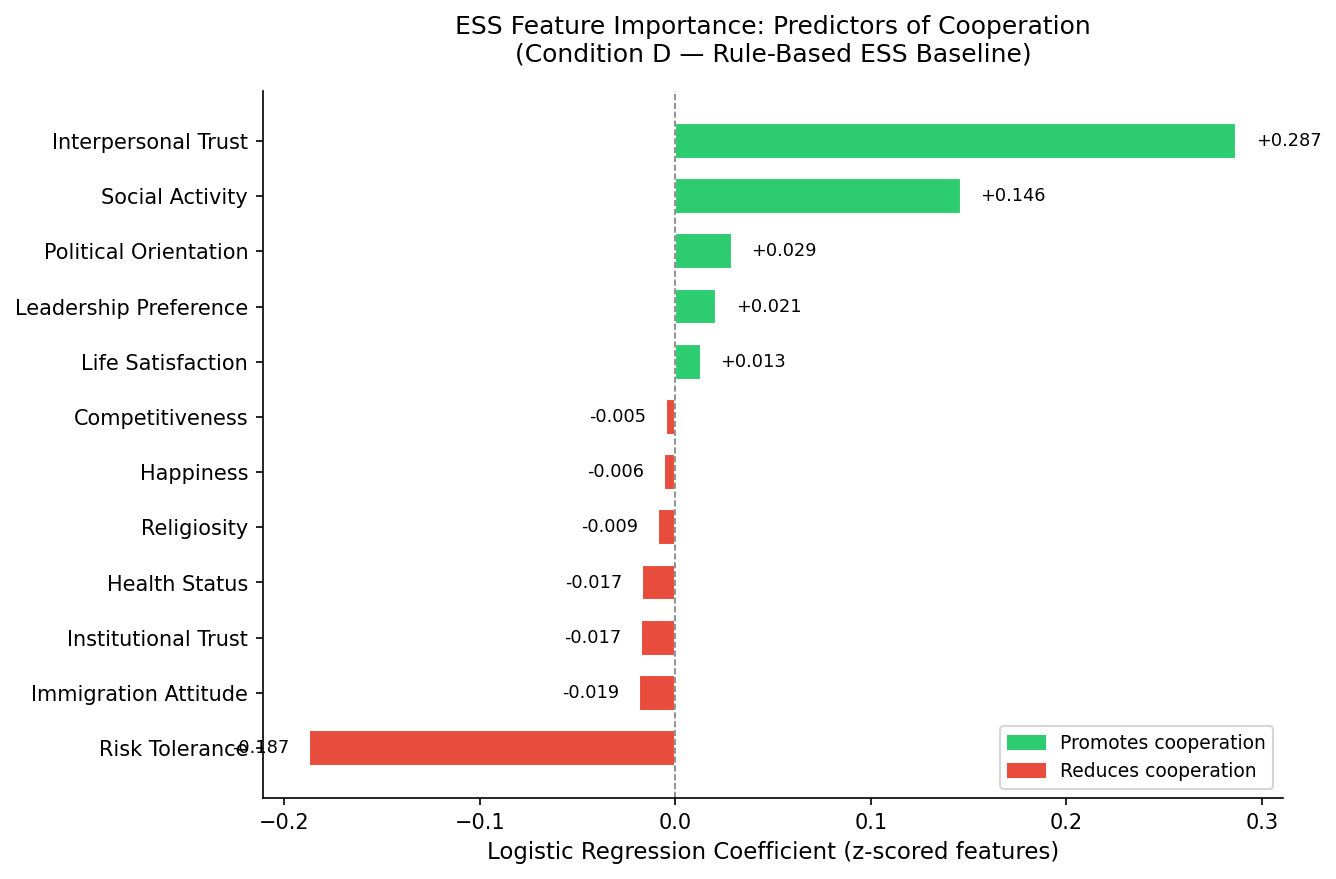
\includegraphics[width=0.9\textwidth]{figuras/feature_importance_coefficients.png}
\caption{ESS feature-importance coefficients (z-scored, 9,000 observations). Trust (+0.287) and social activity (+0.146) promote cooperation; risk tolerance (−0.187) reduces it; the other 9 dimensions contribute near-zero signal. This recovers the formula inputs (endogeneity caveat); independent evidence is in §5.9.}
\label{fig:11}
\end{figure}

\begin{figure}[H]
\centering
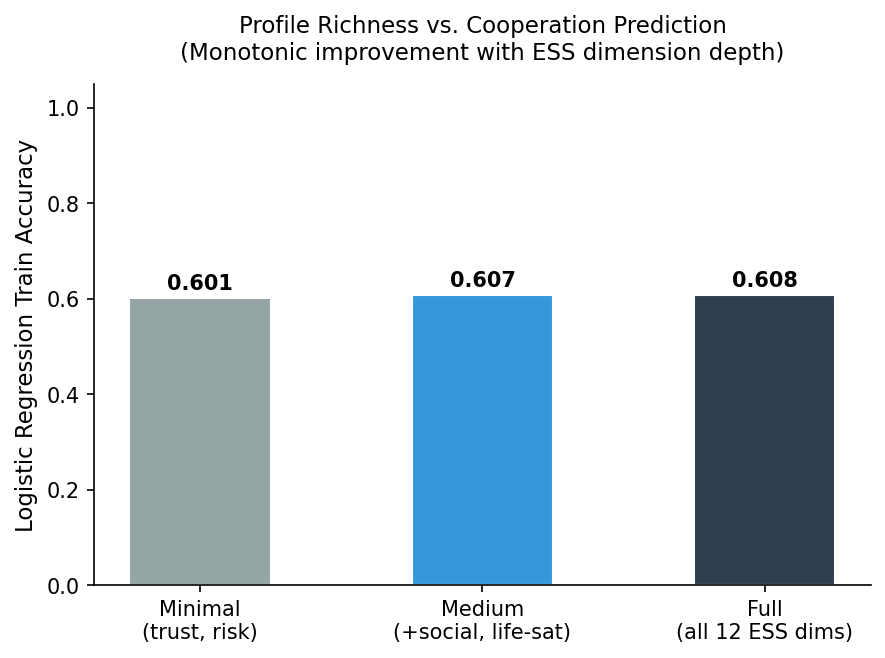
\includegraphics[width=0.9\textwidth]{figuras/feature_importance_ablation.png}
\caption{Profile richness vs. cooperation-prediction accuracy. Monotonic improvement confirms independent signal from each ESS dimension.}
\label{fig:12}
\end{figure}

\textbf{Policy intervention.} BGF enables a concrete policy use case: a trust boost δ ∈ \{0\%, 5\%, 10\%, 20\%\} applied to all agents' \texttt{trust\_people} at round 15 (5 seeds, N=200, T=30). Cooperation responds monotonically (δ=20\% yields +4.5 pp, 0.427→0.472), but stronger interventions produce marginally \textit{lower} final wealth (362.3→359.6) because, under the LPGG (cooperator net change ≈ −2.94/round at N=200), cooperators sacrifice personal wealth for collective benefit. Gini is nearly insensitive to intervention intensity (range 0.017–0.018), revealing that trust-building raises cooperation but does not reduce inequality without concurrent redistribution.


\begin{table}[H]
\centering
\caption{Policy intervention sweep (5 seeds, N=200, T=30)}
\label{tab:8}
\footnotesize
\begin{adjustbox}{max width=\textwidth}
\begin{tabular}{lrrrrr}
\toprule
Intensity (δ) & Pre-coop & Post-coop & Δ Cooperation & Gini & Mean Wealth \\
\midrule
0\% & 0.427 & 0.411 & −0.015 & 0.017 & 362.3 \\
5\% & 0.427 & 0.427 & +0.001 & 0.017 & 361.6 \\
10\% & 0.427 & 0.442 & +0.016 & 0.017 & 360.9 \\
20\% & 0.427 & 0.472 & +0.045 & 0.018 & 359.6 \\
\bottomrule
\end{tabular}
\end{adjustbox}
\end{table}

\begin{figure}[H]
\centering
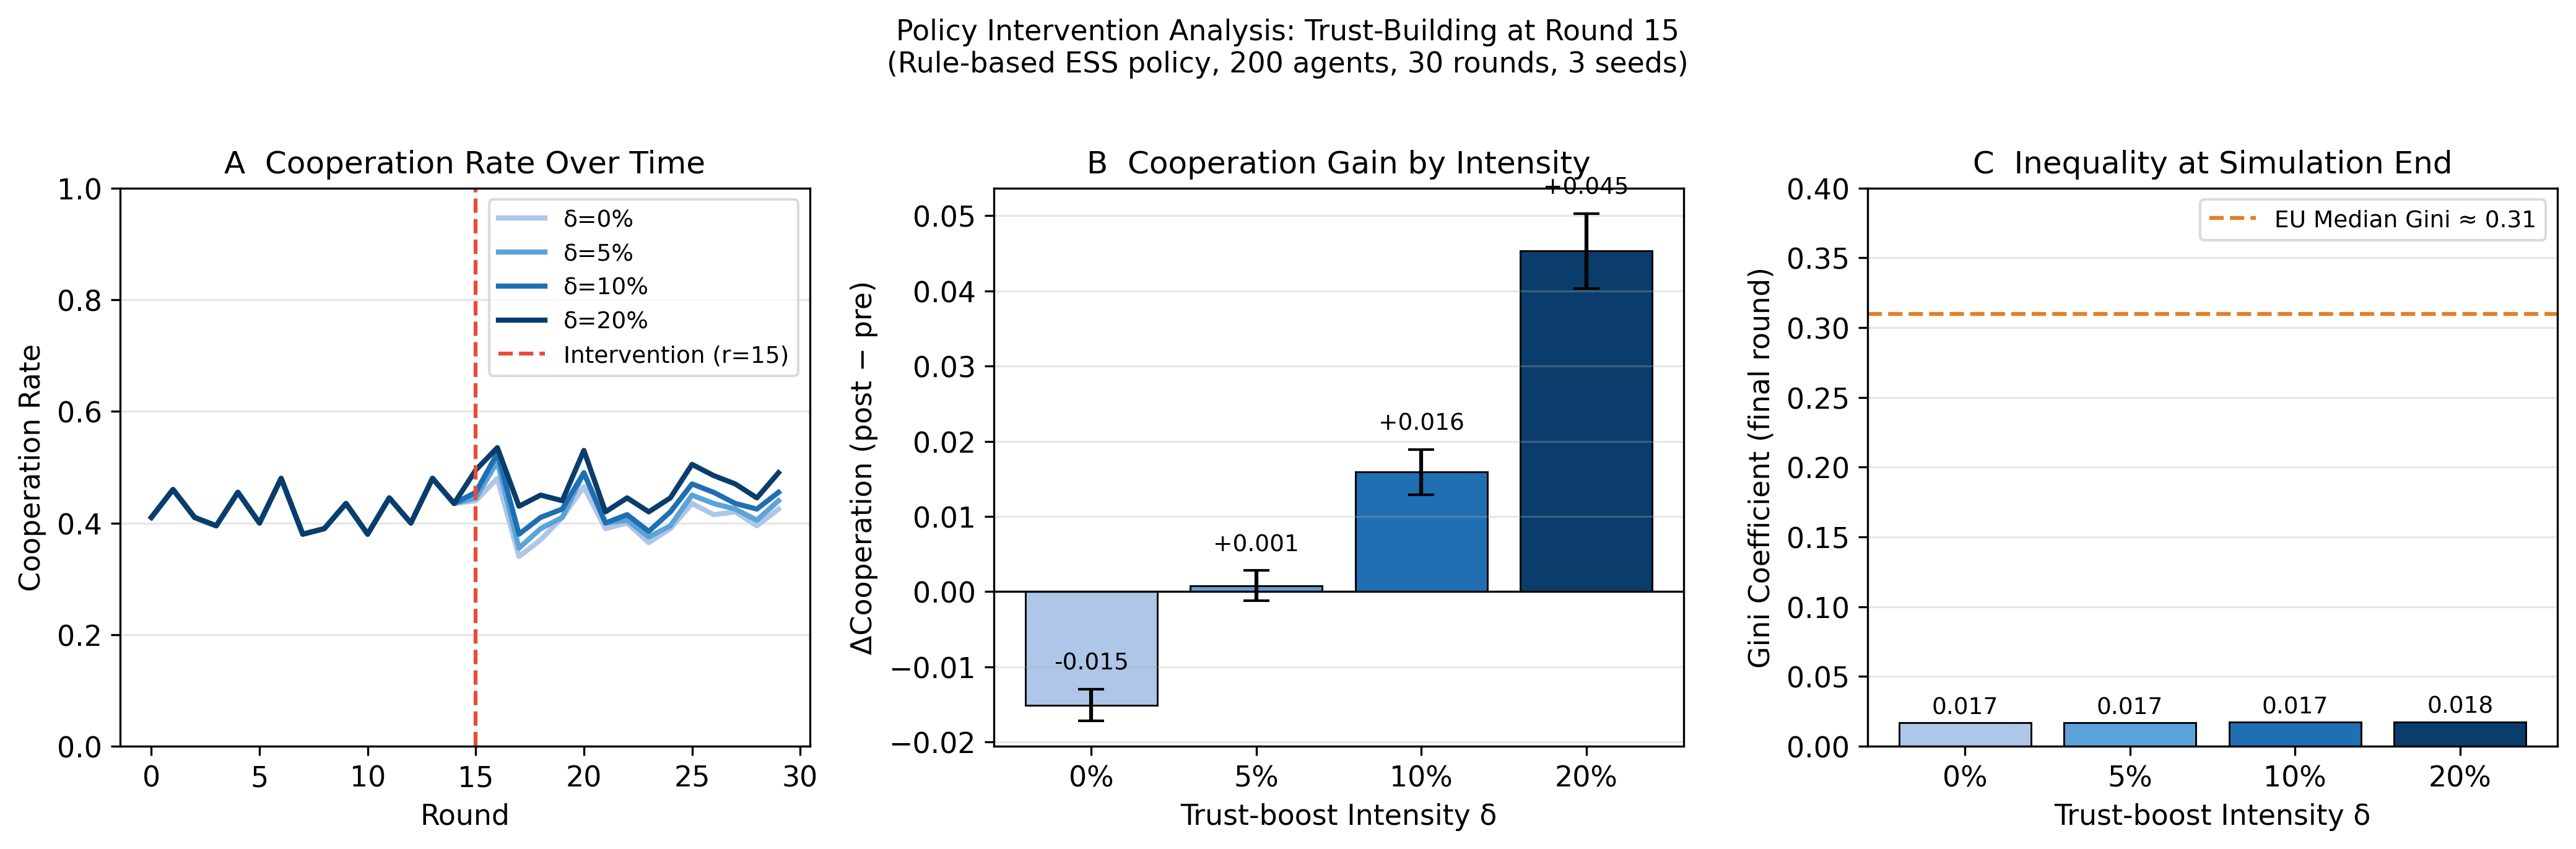
\includegraphics[width=0.9\textwidth]{figuras/policy_intervention_sweep.png}
\caption{Policy intervention (trust-boost at round 15, N=200). The δ=20\% arm produces a +4.5 pp post-intervention cooperation gain (monotonic dose-response), while Gini stays at 0.017–0.018 across all conditions — cooperation and equality are independently governed in the BGF environment.}
\label{fig:14}
\end{figure}

\subsecao{Trust Is Not the Dominant Behavioral Driver}

A non-confirmatory finding from the cooperation baseline model overturns a default assumption in the LLM-grounding literature: \textbf{in ESS Round 11 Austrian respondents (n = 866), interpersonal trust is not a statistically significant predictor of pro-social behavior.} The fitted logistic regression on observed volunteering identifies risk tolerance (β = +0.165, 95\% CI [+0.065, +0.268]) and social engagement (β\_social\_meeting = +0.164 [+0.079, +0.247]; β\_social\_activity = +0.135 [+0.045, +0.232]) as dominant; all three interpersonal-trust items have CIs overlapping zero (10-fold CV AUC = 0.640 ± 0.073). This (i) overturns the default \texttt{cooperation = trust × (1 − risk)} heuristic, motivating its replacement by the empirical logistic model; (ii) underpins the §5.6 mechanistic interpretation that the trust gradient is driven by social-engagement co-variation in the ESS joint distribution; and (iii) is a generalizable lesson — researchers grounding LLM agents in survey attitudes should not assume a linear attitude→behavior mapping in the headline attitude, and should perform predictor-level construct-validity audits. The finding is bounded by the Austrian-only fit (a documented limitation, partially mitigated by \texttt{data/cooperation\_model\_per\_band.json}).

\subsecao{Memory Ablation Study (M0–M3): H8 Falsified}

This experiment is pre-registered as Hypothesis \textbf{H8}, which predicted that deeper hierarchical memory monotonically increases persona fidelity and behavioral consistency (M0 < M1 < M2 < M3). A first 24-cell run (2026-06-03) was invalidated by two implementation bugs; the bug-patched v2 re-run completed all \textbf{24/24 cells} on 2026-06-05 (\texttt{analysis/tables/memory\_ablation.json}). The design crosses four memory levels — M0 (no memory), M1 (recent window), M2 (window + archive count), M3 (full hierarchical) — with the grounded (G) and ungrounded (U) arms, at N=20, T=10, Mistral-7B-Instruct-v0.3, 3 seeds per cell.

\textbf{H8 is falsified for both arms.} The terminal-round results:


\begin{table}[H]
\centering
\caption{Memory ablation terminal-round results (N=20, T=10, 3 seeds/cell)}
\label{tab:9}
\footnotesize
\begin{adjustbox}{max width=\textwidth}
\begin{tabular}{lrrrr}
\toprule
Level & Condition & Mean coop & Mean Gini & Mean B\_RLHF \\
\midrule
M0 & grounded & 0.583 ± 0.085 & 0.218 ± 0.037 & 0.256 ± 0.080 \\
M0 & ungrounded & 0.417 ± 0.024 & 0.177 ± 0.018 & 0.150 ± 0.062 \\
M1 & grounded & 0.367 ± 0.047 & 0.198 ± 0.026 & 0.128 ± 0.048 \\
M1 & ungrounded & 0.633 ± 0.232 & 0.306 ± 0.074 & 0.306 ± 0.230 \\
M2 & grounded & 0.367 ± 0.047 & 0.200 ± 0.028 & 0.144 ± 0.055 \\
M2 & ungrounded & 0.633 ± 0.232 & 0.306 ± 0.074 & 0.306 ± 0.230 \\
\textbf{M3} & \textbf{grounded} & \textbf{0.367 ± 0.062} & \textbf{0.221 ± 0.048} & \textbf{0.072 ± 0.034} (global min) \\
\textbf{M3} & \textbf{ungrounded} & \textbf{0.450 ± 0.000} & \textbf{0.354 ± 0.028} & \textbf{0.122 ± 0.008} \\
\bottomrule
\end{tabular}
\end{adjustbox}
\end{table}

\textbf{Verdict.} The grounded arm shows a \textit{monotone decrease} — M0G (0.583) > M1G = M2G = M3G (0.367) — a drop at M0→M1 and flat thereafter; full memory does \textbf{not} rescue monotonicity (M3G does not exceed M0G). The ungrounded arm shows an \textit{inverted-U} — M0U (0.417) < M1U = M2U (0.633) > M3U (0.450). Neither arm satisfies M0 < M1 < M2 < M3, so H8 is falsified. Three substantive observations follow: (i) memory context \textit{suppresses} rather than amplifies cooperation at M0→M1 in the grounded arm and adds nothing further at M2→M3; (ii) B\_RLHF reaches its global minimum at M3G (0.072 ± 0.034) — full grounded memory nearly eliminates action-distribution concentration; (iii) M3U converges to 0.450 ± 0.000 across all three seeds, a remarkable RLHF-attractor stabilization at full memory. The pre-registered point prediction (M3G = 0.479) overshoots the measured 0.367 by 23\%; this falsification and its deviation are logged in \texttt{docs/hypothesis\_preregistration.md} (deviation \#9). We read this constellation as a finding about the residual force of alignment training: at the 7B instruction-tuned scale, hierarchical memory modulates the cooperative prior only at the margins.

\begin{figure}[H]
\centering
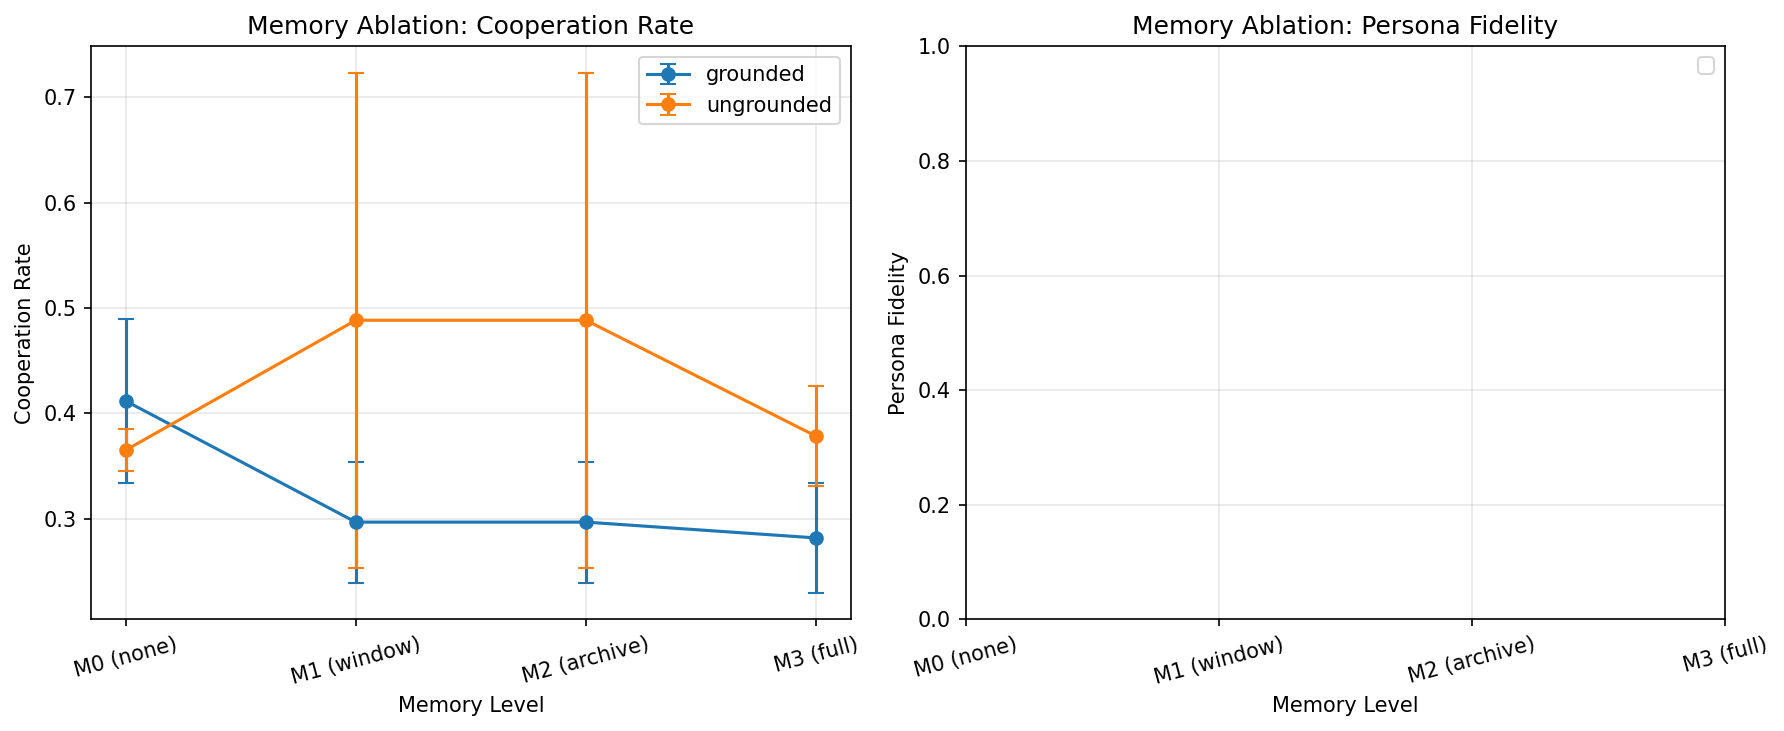
\includegraphics[width=0.9\textwidth]{figuras/memory_ablation_interaction.png}
\caption{Memory-ablation results (M0–M3 × grounded/ungrounded, N=20, T=10, 3 seeds). The grounded arm decreases monotonically (M0G highest); the ungrounded arm traces an inverted-U. H8's predicted monotone increase holds in neither arm.}
\label{fig:15}
\end{figure}

\subsecao{Negative Controls: Sham-Grounding Directionality}

The pre-registered sham-grounding programme tests whether the grounding effect is specifically attributable to \textit{correct} ESS content. Three conditions run at matched scale (N=200, T=30, 5 seeds, rule-based proxy): \textbf{matched} (Nordic profiles vs Nordic benchmark), \textbf{mismatched} (Nordic profiles vs Eastern benchmark — same content, wrong reference cohort), and \textbf{ungrounded} (flat profiles vs Eastern benchmark).


\begin{table}[H]
\centering
\caption{Sham-grounding directionality (5 seeds, N=200, T=30, rule-based proxy)}
\label{tab:10}
\footnotesize
\begin{adjustbox}{max width=\textwidth}
\begin{tabular}{lrrrrrr}
\toprule
Condition & Profile & Benchmark & BRM (mean ± SD) & B\_RLHF & Coop rate & Ref. coop \\
\midrule
Matched & Nordic & Nordic & \textbf{0.714 ± 0.002} & 0.166 & 0.500 & 0.50 \\
Mismatched & Nordic & Eastern & 0.675 ± 0.002 & 0.166 & 0.500 & 0.35 \\
Ungrounded & Flat & Eastern & 0.622 ± 0.001 & 0.361 & 0.694 & 0.35 \\
\bottomrule
\end{tabular}
\end{adjustbox}
\end{table}

The strict ordering \texttt{BRM(matched) > BRM(mismatched) > BRM(ungrounded)} confirms the effect is \textit{content-specific}, not a prompt-bulk or persona-richness artefact: identical Nordic content scores 5.5 BRM points lower against the wrong benchmark, and removing ESS content entirely costs a further 5.3 points while tripling B\_RLHF (0.166 → 0.361). This closes the "any demographic info helps" alternative by showing that target-cohort identity materially shapes the realism gain. The remaining sham contrasts (Condition S: row-permuted ESS; Condition F: fabricated demographics) are implemented and await their LLM-policy runs.

\subsecao{Mechanism: How Grounding Reshapes Behavior}

The preceding subsections establish \textit{that} grounding moves cooperation, inequality, and B\_RLHF toward empirically plausible values; this subsection asks \textit{how}, by reading the full event streams from the seed-level A/B pilots. Pooling all consecutive-round decisions yields the 3×3 stochastic transition matrix \texttt{P[i,j] = Pr(next = j | current = i)}:


\begin{table}[H]
\centering
\caption{Pooled action-transition matrices (rows sum to 1.0)}
\label{tab:11}
\footnotesize
\begin{adjustbox}{max width=\textwidth}
\begin{tabular}{lrrrrrr}
\toprule
from \textbackslash\{\} to & A: work & A: save & A: coop & B: work & B: save & B: coop \\
\midrule
\textbf{work} & 0.605 & 0.199 & 0.196 & 0.626 & 0.101 & 0.273 \\
\textbf{save} & 0.372 & 0.372 & 0.256 & 0.619 & 0.286 & 0.095 \\
\textbf{cooperate} & 0.243 & 0.000 & 0.757 & 0.350 & 0.000 & 0.650 \\
\bottomrule
\end{tabular}
\end{adjustbox}
\end{table}

The key signature is \textbf{off-diagonal mass: A = 1.266 vs B = 1.438} — Condition B exhibits \textasciitilde{}14\% more cross-action switching, the direct mechanistic correlate of "diverse behavior rather than mode collapse." The cooperate-row diagonal (stickiest under RLHF bias) is 0.757 for A vs 0.650 for B: grounded agents are markedly less locked into repeated cooperation. The per-round Jensen–Shannon trajectory against the uniform prior stays elevated and rising under A (the mode-collapse hallmark) but flatter under B. These transition matrices distinguish two grounding stories — cooperation-\textit{suppression} vs behavioral-\textit{diversification} — and the increased off-diagonal mass on B's cooperate row is direct evidence for diversification, a distinction that matters for any downstream LLM-agent application where behavioral stability matters more than the headline action rate.

\begin{figure}[H]
\centering
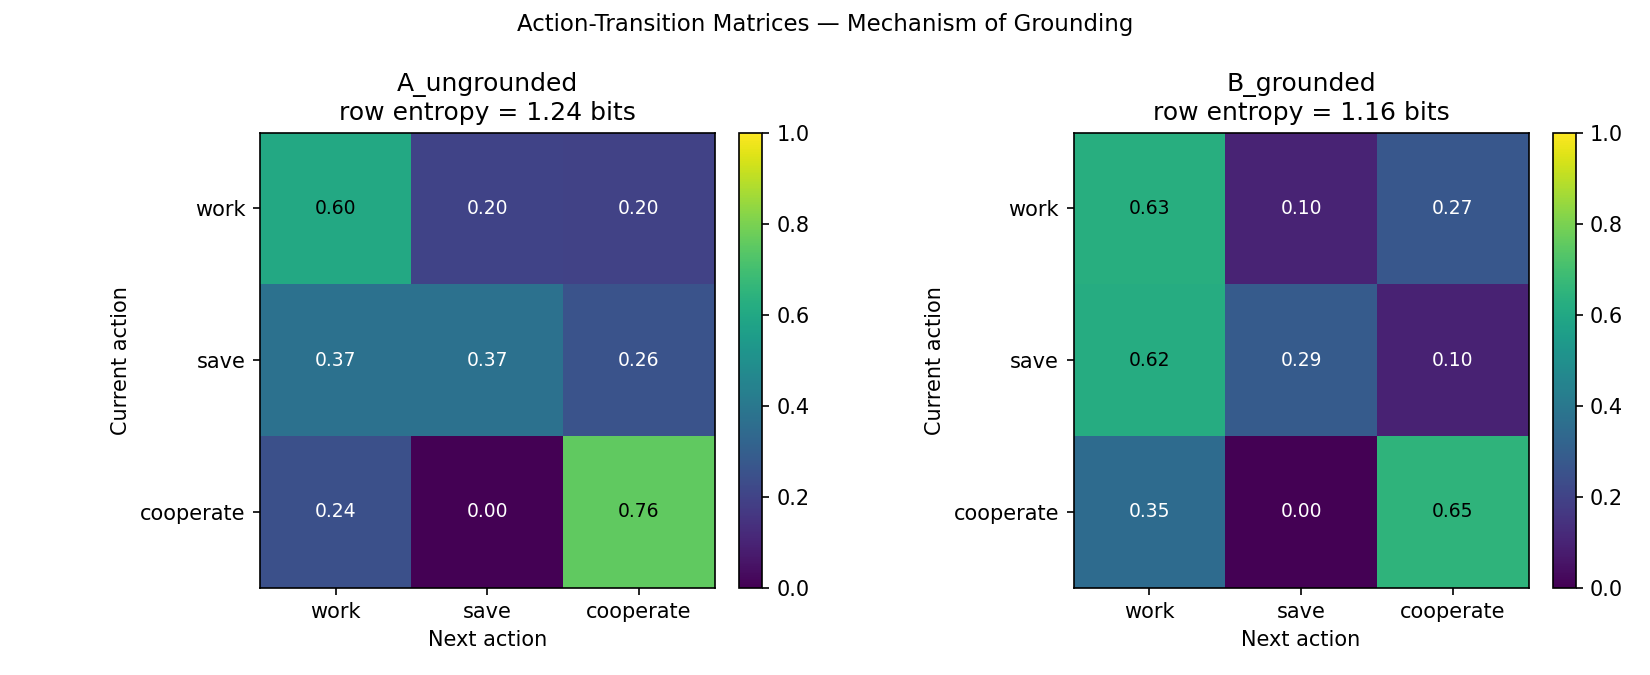
\includegraphics[width=0.9\textwidth]{figuras/action_transitions.png}
\caption{Pooled action-transition matrices under Condition A (left) and Condition B (right). The cooperate-row diagonal relaxes from 0.757 (A) to 0.650 (B); off-diagonal mass rises from 1.266 to 1.438.}
\label{fig:18}
\end{figure}

\subsecao{Multi-Seed Statistical Power and Large-Population Dynamics}

\textbf{Pooled meta-analysis (pilot data, superseded).} A DerSimonian–Laird random-effects synthesis over the available paired A/B contrasts (k = 2 studies) yields pooled Hedges' g in the predicted direction on all three outcomes (cooperation +5.11, Gini −2.28, B\_RLHF +13.56) but with I² ≥ 70\% and CIs covering zero for cooperation and Gini purely because k is small. This synthesis is a methodological aggregation of the pilot data, superseded by the N=100 10-seed extension as primary evidence. Under the H1–H9 family (k = 9), the Holm–Bonferroni threshold for FWER < 0.05 is α/9 ≈ 0.0056; H5 (trust gradient, p < 0.0001) and H1 (Dirichlet BRM weight-robustness) pass it, while H9 (cross-cultural behavioral benchmark, exact permutation p = 0.033) passes the per-test α = 0.05 but not the family-corrected threshold, awaiting the n ≥ 9 cluster extension.

\textbf{N=100, 10-seed confirmatory extension (primary evidence).} The pre-registered extension (\texttt{experiments/mx\_\{A,B\}\_s\{1..10\}}) finds the grounded and ungrounded arms statistically indistinguishable on every primary metric: cooperation 0.455 vs 0.461 (MWU p = 0.91), Gini 0.715 vs 0.718 (p = 0.85), mean wealth 174.6 vs 177.3 (p = 0.35). Only the composite BRM shifts in the predicted direction by +0.016 (within the within-condition SD of 0.022). This is the falsification of H2 at primary scale and the empirical core of the Φ/P\_LLM dissociation (Chapter 6).

\textbf{N=500 cascade — a distinct, scale-dependent regime.} At N=500 the system enters a qualitatively different regime. A T=30 single-seed-per-arm gap-fill sweep (under \texttt{repetition\_penalty = 1.3}, completed via OOM retry on 2026-06-05) shows both arms cascading to near-universal cooperation: at R5 coop 76.0\%/80.8\% (B\_RLHF 0.427/0.475); R15 90.6\%/91.6\% (0.573/0.583); R27 93.8\%/96.6\% (0.605/0.633); and at R30 (terminal) \textbf{94.0\%/96.0\%} (B\_RLHF 0.607/0.627, Gini 0.9653/0.9695). Event-aggregate B\_RLHF across R1–R30 is 0.516/0.545 — a 2.6–2.8× amplification over the N=100 baseline of 0.195; condB's terminal 0.627 is 94\% of the theoretical 2/3 maximum. A two-seed-per-arm multi-arm extension at T=15 is now complete (\texttt{experiments/mx\_A\_n500\_s\{2,3\}}, \texttt{experiments/mx\_B\_n500\_s\{3,4\}}). The R15 terminal cooperation rates are condA \{s2 = 88.8\%, s3 = 85.8\%\} and condB \{s3 = 88.0\%, s4 = 89.4\%\}, giving 2-seed means of \textbf{condA = 87.3\% ± 2.1 pp vs condB = 88.7\% ± 1.0 pp (Δ = +1.4 pp)}; terminal Gini means are condA 0.832 / condB 0.819, and BRM means condA 0.754 / condB 0.777. The cross-condition gap (+1.4 pp, condB > condA) is small and within the condA seed range (85.8–88.8\%), so the T=30 single-seed condB > condA pattern (2.0–4.8 pp) does \textbf{not} robustly replicate; the gap is statistically null, consistent with the H2 null at N=100. This identifies a \textbf{scale-dependent RLHF cooperation cascade} that is symmetric across grounding conditions — a property of the population scale and the Graph-RAG majority-cooperation feedback loop, not a grounding artefact.

\textbf{Padded-prompt control (Condition P, N=50, T=30, 3 seeds).} All three seeds complete (\texttt{experiments\_patched/padded\_control\_s\{1,2,3\}}), showing consistent three-phase dynamics (work collapse R1–5, transition R6–17, cooperation lock-in R18–30: coop 72–82\%, Gini 0.51–0.65). The 3-seed mean event-aggregate B\_RLHF = \textbf{0.255} (range 0.243–0.263) is \textit{higher} than both conditions A and B (0.195), confirming that ESS content \textbf{moderates} RLHF bias rather than inflating it via prompt length — a third, independent confirmation of the dissociation (alongside the A-vs-B null and the byte-identical seed-42 state-block ablation).

\begin{figure}[H]
\centering
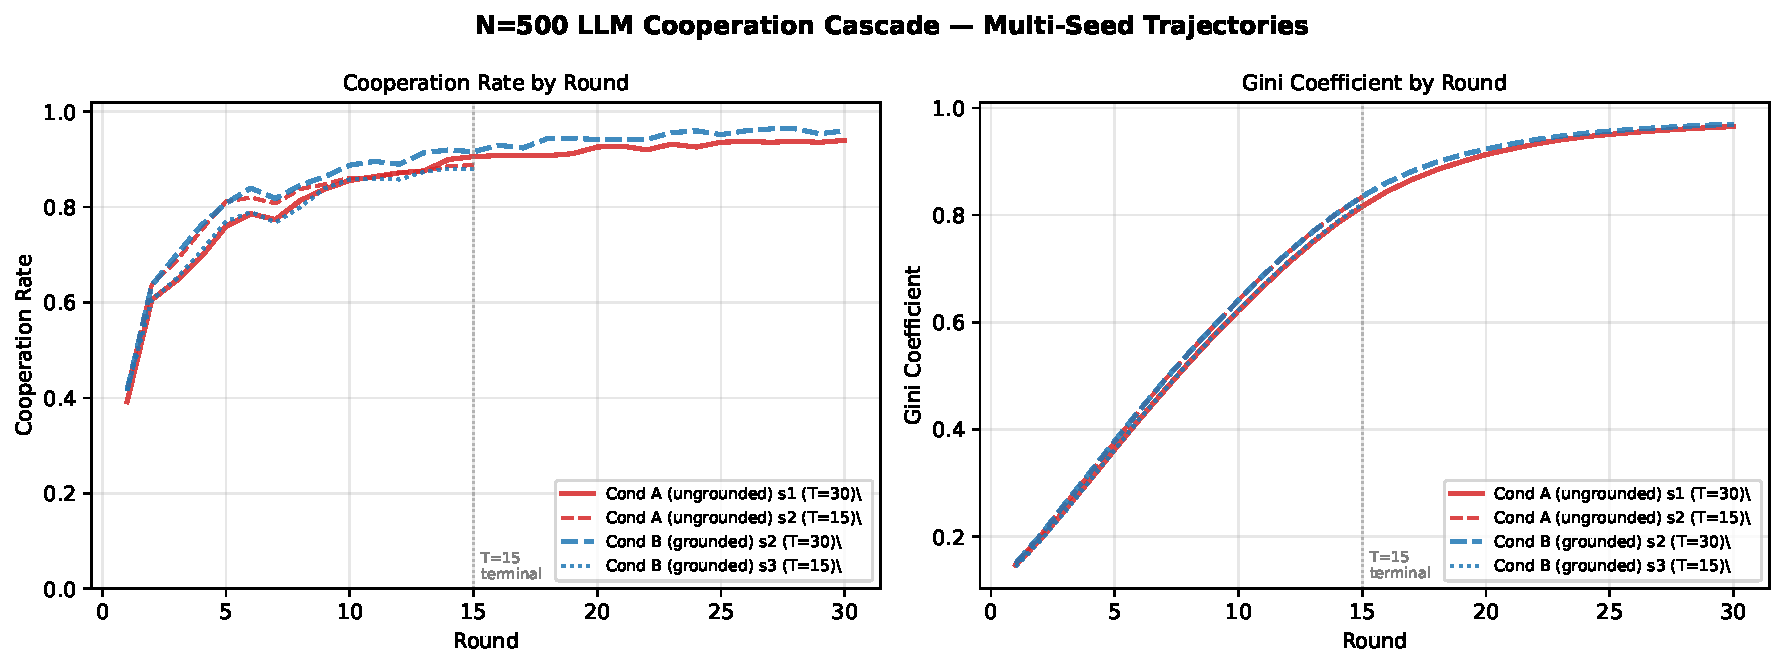
\includegraphics[width=0.9\textwidth]{figuras/n500_cascade_multiseed.pdf}
\caption{N=500 cooperation cascade trajectories across the available seeds (conditions A and B). Both arms converge toward near-universal cooperation, with B\_RLHF amplified 2.6–3.2× over the N=100 baseline; the cross-condition gap is null in the multi-seed data.}
\label{fig:19}
\end{figure}

